\section{Patterns 6 - Model-View-ViewModel (MVVM)}

\subsection{Fokuspunkter}

\begin{itemize}
	\item Redegør for, hvad et software pattern er.
	\item Redegør for Model-View-ViewModel mønstret og dets variationer.
\end{itemize}

\subsection{Hvad er et Software pattern?}

\derp

Dette design pattern, er et GUI architecture pattern, som er en specaialisering af Model-View-Presenter møsntret.

\subsection{Redegør for Model-View-ViewModel mønstret og dets variationer}

\begin{figure}[h]
	\centering
	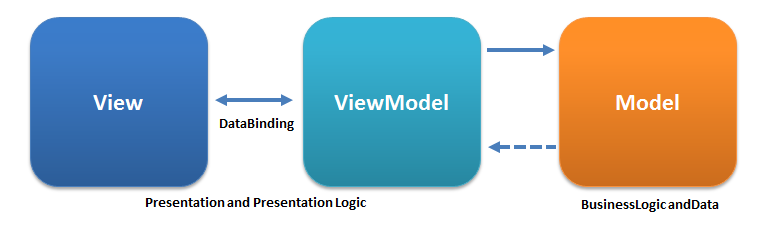
\includegraphics[width=0.7\linewidth]{figs/MVVM/MVVMPattern.png}
	\caption[Sammenhæng mellem Model-View-ViewModel]{}
	\label{fig:MVVMPattern}
\end{figure}

\subsubsection{View}

\begin{enumerate}
	\item User Interface.
	\item Definerer struktur, layout og appearance.
	\item Ideelt er det udelukkende defineret i XAML, med begrænset "code behind" som \textbf{\textit{ikke}} indeholder business logic.
	\item Kan være en subcomponent af et andet view.
	\item Kan have sin egen ViewModel eller arve dens parents.
	\item Viewet får data fra ViewModel gennem \textbf{\textit{databinding}} eller metodekald på ViewModel
	\item View ændres \textbf{\textit{run-time}} når UI controls\todo{GUIPERSON: what is dis?}, agerer efter ændringer i ViewModels properties.
	\item Hvad sker der der laves User Input på View?
	\begin{itemize}
		\item Hvis control er en \textbf{\textit{Command Source}} kan control's Command property være data bound til en ICommand property på view model.
		\item View er connected til ViewMOdel gennem databinding og sender commands to ViewModel
	\end{itemize}
\end{enumerate}

\subsubsection{ViewModel}
\begin{enumerate}
	\item \textbf{En model af Viewet}.
	\begin{itemize}
		\item En abstraktion af viewet der leverer \textbf{data binding} mellem View og Model
		\item En specialiseret udgave af MVP's presenter (agerer også \textit{converter} der omdanner Model data til View data), og samtidig overfører commands fra View til Model.
	\end{itemize}
	\item ViewModel har \textbf{\textit{public}} properties og commands.
	\item  Interagerer med Model gennem Databinding, properties og metodekald.
	\item Modtager events fra Model
\end{enumerate}

\subsubsection{Model}
\begin{enumerate}
	\item Refererer som i MVC til enten:
	\begin{itemize}
		\item Object-model, der repræsenterer state content.
		\item Data Access layer der repræsenterer indhold.
	\end{itemize}
	\item \textbf{Kender ikke til ViewModel}\todo{GUIPERSON: hvordan sender den events?}
	\item Sender evnets til ViewModel
\end{enumerate}

\subsubsection{Commands}
Data binding af View til Properties i ViewModel fungerer ganske fint og kan sagtens lade sig gøre. Data binding til funktioner er dog ikke muligt, selvom det ofte er til nytte. Data binding til funktionskald er f.eks. brugbart til en ”Gem”-knap, som skal gemme en række data, når brugeren trykker på knappen.
For at kunne data binde til en funktion kan der bruges ”RelayCommand”. RelayCommand er udviklet af Josh Smith. Et alternativ kan være ”DelegateCommand” fra Prism frameworket. RelayCommand er brugt i GUI-kurset.
RelayCommand fungerer således, at der laves en Command property, som View kan data binde til. Commanden ”relayer” til en metode, og når en knap der er data bindet til en command bliver trykket på, så vil den pågældende metode blive kaldt. På denne måde kan der data bindes til metoder.

\subsubsection{Oprettelse af Views og ViewModels}
\textbf{To måder}:
\begin{enumerate}
	\item \textbf{View First} - Viewet laves først og en ViewModel kobles efterfølgende på, ved at denne oprettes fra viewet. Dette kan gøres på forskellige måder – eksempler følger.
	\item \textbf{ViewModel First} - ViewModel laves først, og det view der hører til ViewModel findes efterfølgende og vises til brugeren. Denne metode er lidt mere kompliceret. Eksempel følger.
\end{enumerate}

\paragraph{View first - ViewModel oprettes i codeBehind}

\begin{lstlisting}[caption=ViewModel oprettes i views codeBehind]
public MainWindow()
{
	InitializeComponent();
	DataContext = new ViewModel(new Model)
}
\end{lstlisting}


\begin{figure}[H]
\centering
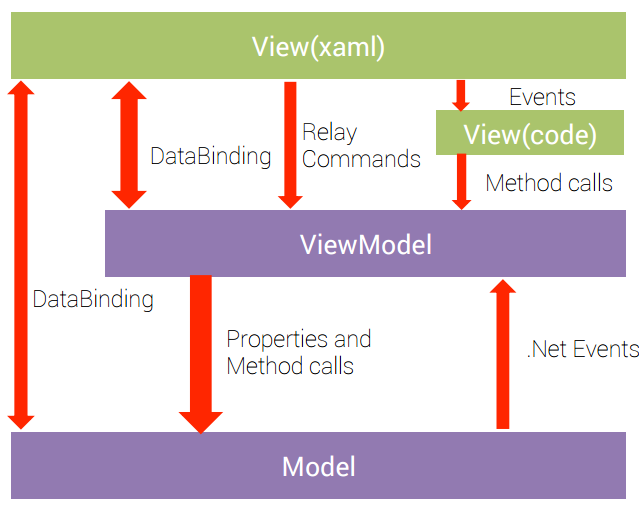
\includegraphics[width=0.7\linewidth]{figs/MVVM/mvvmPatternComplex}
\caption{Intern adfærd i MVVM pattern}
\label{fig:mvvmPatternComplex}
\end{figure}

\subsubsection{Hvorfor er det smart?}

\begin{itemize}
	\item \textbf{Test uden UI} - UI indeholder ikke business logic.
	\item 
\end{itemize}




